%! Author = adnansiddiquei
%! Date = 13/12/2023

\subsection{Dataset A}\label{subsec:dataset-a}
\subsubsection{Question 1a}\label{subsubsec:q1a}
    \begin{figure}[htb]
    \centering
    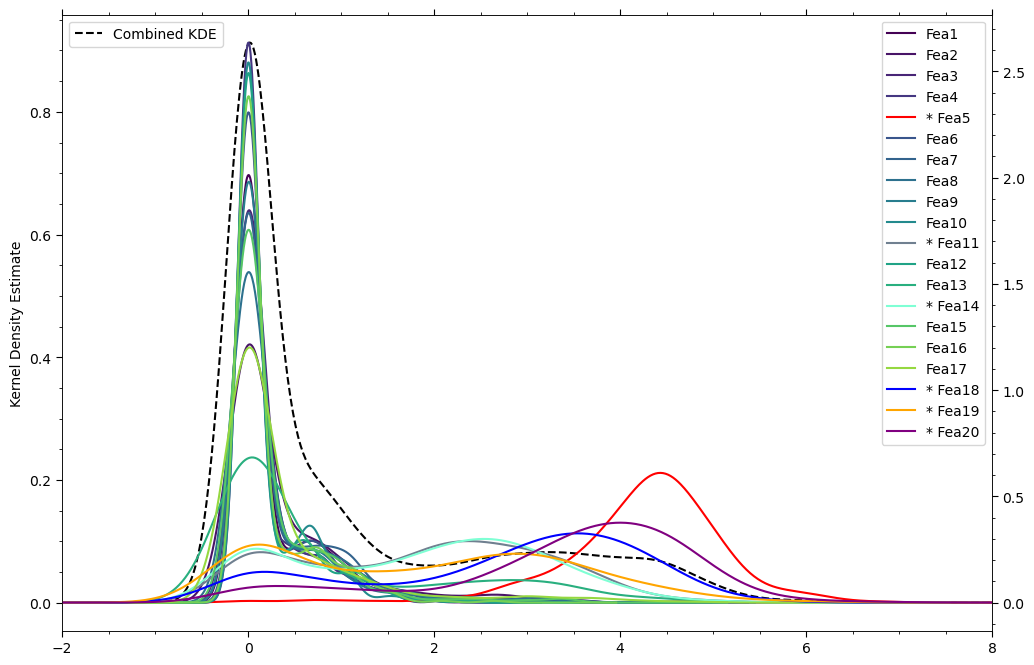
\includegraphics[width=0.9\textwidth]{./figures/q1a}
    \caption{A kernel density estimate of the first 20 features of the \inlinecode{A_NoiseAdded.csv} dataset, which has 20
    plots in total, with the legend and corresponding y-axis on the right. A combined KDE has also been plotted, with
    it's corresponding x-axis on the left. 7 of the 20 features have been highlighted in the legend with an asterisk,
    and have been coloured in slightly more contrasting colours and plotted with a dotted line. These features have a
    larger variance in their density, and are therefore more likely to be more discriminative.}
    \label{fig:q1a}
    \end{figure}

    Fig\eqref{fig:q1a} shows the combined and separated kernal density estimates of the first 20 features of the dataset.
    Several conclusions can be drawn from this plot.
    For most of the features, the KDE is concentrated around the zero value with very little variance, with the exception
    of 7 features: 5, 11, 13, 14, 18, 19 and 20.
    These features are likely to be more discriminative within classification algorithms, as they contain more variability.

\subsubsection{Question 1b}\label{subsubsec:q1b}

    \begin{figure}[htb]
    \centering
    \begin{subfigure}[b]{0.9\linewidth}
        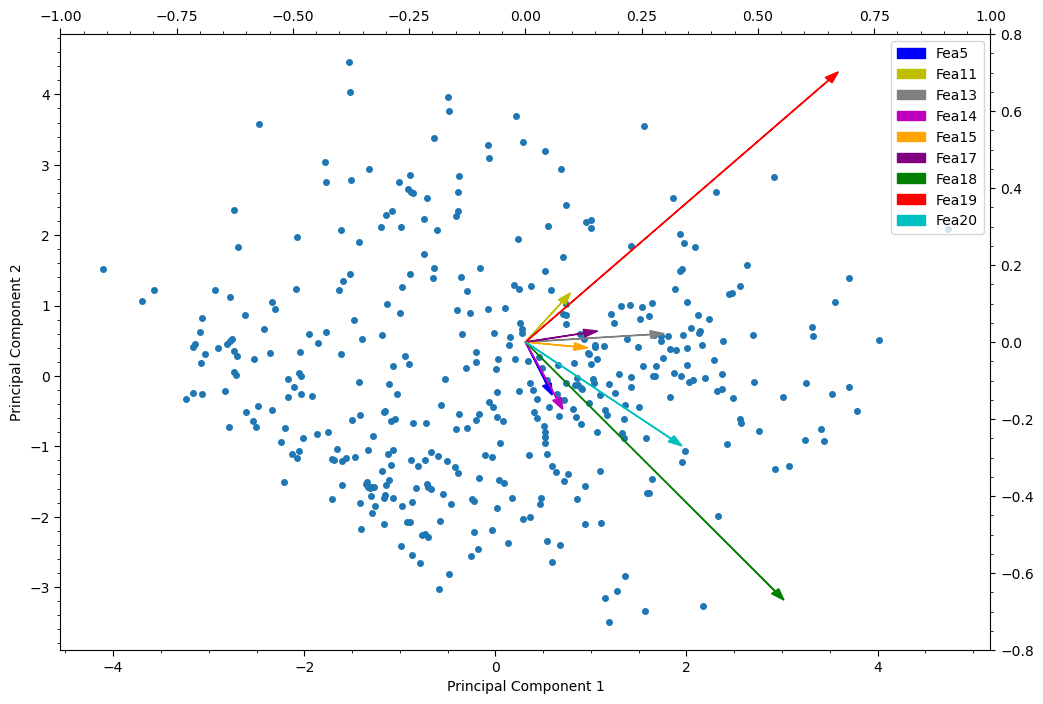
\includegraphics[width=0.9\textwidth]{figures/q1b-1}
        \caption{A biplot of the first two principal components in the dataset.
        The arrows indicate the first two principal component loading vectors for every feature which contributes to
        either principal component more than 1\%. The loading vectors use the right and top axis of the plot. The blue dots
        indicate the scores for each observation in the dataset for the first two principal components.}
        \label{fig:q1b-1}
    \end{subfigure}
    \hfill
    \begin{subfigure}[b]{0.9\linewidth}
        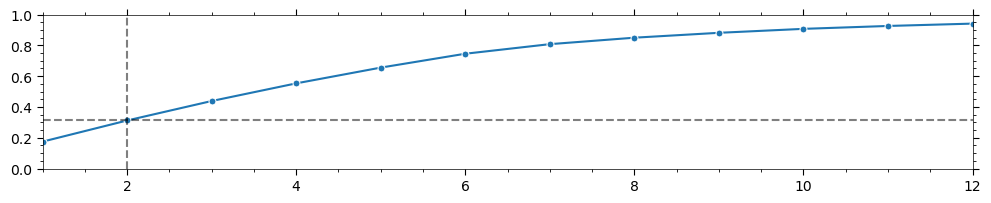
\includegraphics[width=0.9\linewidth]{figures/q1b-2}
        \caption{A line plot of the explained variance ratio for the first 12 principal components.}
        \label{fig:q1b-2}
    \end{subfigure}
    \caption{Two plots illustrating the results of a PCA of the first 20 features of the \inlinecode{A_NoiseAdded.csv}
    dataset.}
    \label{fig:q1b}
    \end{figure}

    Fig\eqref{fig:q1a} indicates that the features are all on a similar scale, so the features do not need to be scaled
    before applying PCA.
    The biplot in Fig\eqref{fig:q1b-1} shows a PCA of the first 20 features of the dataset, as predicted, the 7 features
    identified in the Fig\eqref{fig:q1a} are the most discriminative, as they are amongst the 9 features in the biplot
    that contribute more than 1\% to either principal component.
    Features 18 and 19 are the most discriminative, as they contribute the most to the principal components.
    However, Fig\eqref{fig:q1b-2} shows the explained variance ratio for the first 12 principal components, and it can
    be seen that the first 2 principal components with the first 20 features only explain 31.2\% of the variance in the dataset.
